\section{Evaluation}
\label{cha:evaluation}
\subsection{Evaluation Setup}
\label{sec:evaluation_setup}
\subsubsection{Infrastructure}
\label{sec:evaluation_infrastructure}
The experiments were conducted on a single-node system equipped with an AMD EPYC 8224P 24-core, 48-thread processor and 188 GB of RAM. The processor supported simultaneous multithreading and frequency boosting up to 2.55 GHz, with 64 MB of shared L3 cache and a single NUMA domain ensuring uniform memory access across all cores. Storage was provided by a 3.5 TB NVMe SSD, and the system ran a 64-bit Linux environment configured for stable and reproducible execution.
To collect accurate power usage data, the node was connected to a 12-way switched and outlet-metered PDU (Expert Power Control 8045 by GUDE), which provided per-outlet power measurements via a REST API.

% TODO: 
\subsubsection{Workflows}
\label{sec:evaluation_workflows}
% TODO: Add correct values there
% Table with different workflows and their characteristics
\begin{table}[H]
    \centering
    \caption{Overview of evaluated nf-core workflows and their inputoutput characteristics.}
    \label{tab:workflow_overview}
    \renewcommand{\arraystretch}{1.15}
    \resizebox{\textwidth}{!}{
        \begin{tabular}{
            p{3.5cm}
            >{\centering\arraybackslash}p{3cm}
            >{\centering\arraybackslash}p{3cm}
            >{\centering\arraybackslash}p{3cm}
            >{\centering\arraybackslash}p{3cm}
            }
            \toprule
            \textbf{Workflow}     & \textbf{Number of Tasks} & \textbf{Input Files} & \textbf{Output Files} & \textbf{Data Profile}                                    \\
            \midrule
            \texttt{atacseq}      & 72                       & 24                   & 185                   & Bulk chromatin accessibility sequencing (ATAC-seq)       \\
            \texttt{chipseq}      & 68                       & 22                   & 172                   & Bulk chromatin immunoprecipitation sequencing (ChIP-seq) \\
            \texttt{rnaseq}       & 54                       & 18                   & 160                   & Bulk RNA-seq expression quantification                   \\
            \texttt{scnanoseq}    & 83                       & 25                   & 210                   & Single-cell nanopore RNA-seq                             \\
            \texttt{smrnaseq}     & 59                       & 20                   & 142                   & Small RNA sequencing (miRNA/siRNA profiling)             \\
            \texttt{pixelator}    & 44                       & 16                   & 125                   & Spatial transcriptomics pixel-based expression mapping   \\
            \texttt{methylseq}    & 65                       & 21                   & 170                   & Whole-genome or targeted DNA methylation sequencing      \\
            \texttt{viralrecon}   & 51                       & 19                   & 150                   & Viral genome assembly and variant analysis               \\
            \texttt{oncoanalyser} & 97                       & 28                   & 260                   & Comprehensive somatic cancer genome analysis             \\
            \bottomrule
        \end{tabular}
    }
\end{table}

\subsubsection{Monitoring Configuration}
\label{sec:evaluation_monitoring_configuration}
% Table with different combinations

\begin{table}[H]
    \centering
    \caption{Adaptable Monitoring Configuration Overview.}
    \label{tab:monitoring_config_overview}
    \renewcommand{\arraystretch}{1.15}
    \resizebox{\textwidth}{!}{
        \begin{tabular}{
            p{3.5cm}
            >{\centering\arraybackslash}p{2cm}
            p{5cm}
            p{6cm}
            }
            \toprule
            \textbf{Monitoring Target} & \textbf{Enabled} & \textbf{Supported Data Sources}                         & \textbf{Collected Metric Types / Adaptability Notes}                                                                    \\
            \midrule

            Task Metadata              &                  & slurm-job-exporter                                      & Collects job metadata (state, runtime, working directory). Can adapt to other job schedulers.                           \\

            CPU                        &                  & cAdvisor, ebpf-mon, docker-activity                     & Captures CPU time and cycles from both container and kernel levels. Supports switching sources for varying granularity. \\

            Memory                     &                  & cAdvisor, docker-activity                               & Tracks memory utilization at container or process level. Configurable for byte- or percentage-based metrics.            \\

            Disk                       &                  & cAdvisor                                                & Monitors block I/O and filesystem throughput. Supports extension with storage exporters.                                \\

            Network                    &                  & cAdvisor (optional)                                     & Disabled by default due to noise. Can be enabled for network-intensive workflows.                                       \\

            Energy                     &                  & docker-activity, ebpf-mon, ipmi-exporter, snmp-exporter & Multi-layer energy monitoring from container to node level. Adaptable to hardware sensors and external power meters.    \\

            \midrule
            \multicolumn{4}{l}{\textbf{Prometheus Configuration}}                                                                                                                                                                             \\[3pt]
            \multicolumn{4}{p{16.5cm}}{
                The Prometheus backend collects all metrics via configurable scrape intervals and targets. Controller and worker nodes can be flexibly defined, enabling distributed monitoring setups.
            }                                                                                                                                                                                                                                 \\

            \bottomrule
        \end{tabular}
    }
\end{table}

\subsubsection{Implemented Models for Task Clustering and Prediction}
\label{sec:evaluation_statistical_learning_methods}
% TODO: Add references to the chapters.
As described in Chapter 5, the statistical models—including the clustering and prediction components—are provided through a FastAPI implementation, allowing external simulation engines to interact with them programmatically. At the same time, the core functionality of the coloc-app FastAPI service is based on a Jupyter Notebook that contains all implementations of the clustering and predictive models discussed in Chapter 5. Both the notebook and the coloc-app were executed on the host system described in Section %\ref{sec:evaluation_infrastructure}.

\subsubsection{Simulation Setup}
\label{sec:evaluation_simulation}

\paragraph{Simulated Platform Configuration}
The infrastructure described in Section \ref{sec:evaluation_infrastructure} was replicated within the SimGrid simulation environment using its platform description tool, as shown in the following XML configuration. The hosts core performance was calibrated by executing stress-ng benchmarks to determine realistic CPU speeds, while network throughput was measured using sysbench. To determine power states (P-states), the GUDE power meter was used to record power consumption in both idle and active conditions under varying load profiles generated with stress-ng. This procedure ensured that the simulated environment accurately reflected the performance and energy characteristics of the physical test system.

% Platform XML file 
\lstinputlisting[
    language=XML,
    caption={Example XML Configuration File},
    label={lst:xml_config}
]{/home/nfomin3/dev/ThesisDocument/fig/06/siena_cluster.xml}

\paragraph{Baseline Scheduling Algorithms}

To evaluate the effectiveness of the proposed approach, we compare it against a series of progressively refined baseline algorithms that address the co-location problem with increasing complexity. These baselines range from simple scheduling heuristics to more advanced strategies that gradually incorporate awareness of co-location effects. The following table summarizes all baselines considered in this study. It is important to note that while some of them already involve concurrent execution of tasks, this represents uncontrolled co-location rather than informed or optimized placement. For clarity and conciseness, detailed algorithmic designs of these baselines are provided in the appendix, while this section focuses on describing their conceptual behavior.

% Overview table over all baselines
\begin{table}[H]
    \centering
    \caption{Overview of Baseline Scheduling Algorithms.}
    \label{tab:baseline_overview}
    \begin{tabularx}{\textwidth}{l l X}
        \toprule
        \textbf{Algorithm} & \textbf{Type}                                & \textbf{Description}                                                                                                          \\
        \midrule
        Baseline 1         & FIFO + Round-Robin                           & Executes tasks in FIFO order and assigns them to hosts in a round-robin fashion without co-location or backfilling.           \\

        Baseline 2         & FIFO + Backfilling                           & Assigns tasks in FIFO order to the first available host, allowing idle hosts to be backfilled opportunistically.              \\

        Baseline 3         & FIFO + VM Co-location                        & Groups multiple ready tasks on the same host within a single VM if sufficient resources are available.                        \\

        Baseline 3.1       & Max-Core VM Co-location                      & Prefers the host with the largest number of idle cores for task co-location to maximize utilization.                          \\

        Baseline 3.2       & Max-Parallel VM Co-location                  & Distributes ready tasks across all available hosts in parallel, promoting high concurrency across nodes.                      \\

        Baseline 4         & VM Co-location + Over-Subscription           & Extends co-location by allowing controlled CPU over-subscription on selected hosts using an oversubscription factor $\alpha$. \\

        Baseline 4.1       & Max-Parallel Co-location + Over-Subscription & Combines parallel host utilization with co-location and controlled CPU over-subscription for improved throughput.             \\
        \bottomrule
    \end{tabularx}
\end{table}

% TODO: Make font distinct from the baselines.
% W/O Co-location
% Baseline 1
The baseline scheduling algorithm implements a simple, sequential execution model designed to simulate isolated task processing within a virtualized cluster. The scheduling process is divided into three abstract components that operate in a fixed order: task scheduling, node assignment, and resource allocation. The scheduler applies a first-in, first-out (FIFO) policy, maintaining a queue of workflow tasks sorted by their readiness. Tasks are retrieved from this queue strictly in order of arrival, preserving dependency constraints and ensuring a fully deterministic execution sequence without reordering or prioritization.
Once a task is selected for execution, the node assignment component distributes it across available compute hosts using a round-robin policy. This mechanism cycles through hosts in sequence, ensuring an even and systematic distribution of tasks across the cluster. No host is assigned more than one active task at a time, enforcing exclusive execution and preventing contention for shared resources.
% Baseline 2
The next variant keeps the same FIFO scheduler and VM-based allocator as Baseline 1, but replaces exclusive node assignment with a greedy backfilling policy. Tasks are still dequeued strictly in arrival order by the FIFO scheduler. For each ready task, the node assignment component queries the cluster for the current number of idle cores per host and performs a first-fit scan: it selects the first host that reports at least one idle core, without requiring the host to be completely idle. The allocator then provisions a VM on the chosen host, binds the tasks inputs/outputs, submits the job to that VM, and on completion shuts the VM down and destroys it.
Conceptually, this turns the placement step into gap filling rather than strict exclusivity. Multiple tasks can be co-located on the same host up to its core capacity, increasing instantaneous parallelism and utilization.
% With co-location
% Baseline 3
Baseline 3 does not differ in the scheduling behavior but replaces the standard allocator and node assignment with components that allow for co-location. When the node assignment component queries the cluster for idle-core availability, it again selects the first host with available cores. However, instead of launching one VM per task, all ready tasks that fit within the hosts idle-core capacity are grouped into a single batch. These tasks are then co-located inside one shared VM instance that is dimensioned according to the aggregate resource requirements of the batch—its vCPU count and memory size are computed as the sum of the respective task demands.
Conceptually, this baseline captures the behavior of intra-VM co-location, where multiple independent tasks share the same virtual machine instead of being distributed across separate ones.
% Baseline 3.1
Baseline 3 is extended by 2 variants where the first one extends thenode assignment component to query the cluster for idle-core availability and selects the host with the maximum amount of available cores. However, instead of launching one VM per task, all ready tasks that fit within the hosts idle-core capacity are grouped into a single batch. These tasks are then co-located inside one shared VM instance that is dimensioned according to the aggregate resource requirements of the batch—its vCPU count and memory size are computed as the sum of the respective task demands.
% Baseline 3.2
The second extension replaces the placement policy with a selection step for the host with maximum idle cores. At each dispatch, the node-assignment component queries the cluster for the current idle cores per host map and picks the host with the largest number of free cores. It then forms a batch by taking as many ready tasks from the FIFO head as the chosen host can accommodate. Compared to first-fit co-location, it tends to reduce residual fragmentation by packing work onto the most spacious node, while still honoring FIFO ordering and leaving task runtime/I/O handling unchanged.
% Baseline 4
The 4th baseline retains the same FIFO scheduler but introduces a node assignment and allocation policy focused on maximizing parallel host utilization. Upon each scheduling cycle, the node assignment component queries the cluster for the current number of idle cores per host, filters out fully occupied nodes, and ranks the remaining hosts in descending order of available cores. It then assigns tasks in batches, filling the host with the highest idle capacity first and grouping as many ready tasks as the hosts idle-core count allows. Once the first host is filled, the process continues with the next host until all tasks in the ready queue are mapped.
The allocator provisions one VM per host batch, sizing it to match the aggregate requirements of all tasks assigned to that host. The resulting VMs vCPU and memory configuration reflect the total core and memory demands of the batch. Each task in the batch is submitted as an independent job to the same virtual compute service, and the VM remains active until all its co-located tasks have finished, at which point it is shut down and destroyed.
% Baseline 4.1
The last baseline extends the previous one by allowing controlled CPU over-subscription during co-location.
At each scheduling cycle, the node assignment component queries per-host idle cores, sorts hosts in descending idle capacity, and fills the largest host first. Unlike the non-oversubscribed version, the per-host batch may exceed the currently idle cores by a fixed factor the batch limit is set to. The procedure continues down the ranked host list, forming one batch per host in the same cycle.
The allocator provisions one VM per host batch, but caps the VMs vCPU count to the hosts actual idle cores at allocation time not the sum of task core demands, while sizing memory to the aggregate of the batched tasks. All tasks in the batch are then submitted to that single VM and execute concurrently on a vCPU pool intentionally smaller than their combined declared cores. The VM remains active until all co-located tasks complete, then it is shut down and destroyed.
Crucially, the degree of contention—and thus realized speedup or slowdown—depends on the complementarity of the co-located task profiles. When CPU-, memory-, and I/O-intensive phases overlap unfavorably oversubscription amplifies interference and queueing on scarce vCPUs. When profiles are complementary, the same oversubscription admits more useful overlap with less contention, improving per-host throughput. Conceptually, this variant implements parallel, capacity-ranked co-location with controlled oversubscription.

\subsection{Experiment Results}
\label{sec:experiment_results}
The section on experimental results is organized as follows. We begin with a brief discussion of the monitoring results obtained using the configuration described earlier. Next, we revisit the approach introduced in Chapter 4 by examining the workload experiments and the resulting measurements that form the basis for subsequent evaluation steps. We then present the outcomes of the statistical methods applied in this work, starting with an in-depth analysis of the task consolidation approach introduced in Chapter 4. Building on these results, we continue with an interpretation of the outcomes from training two predictive models on the clustering data. Finally, we integrate all components into a unified simulation framework. Using this setup, we execute all workflows introduced at the beginning of Chapter 6 with the algorithms detailed in Chapter 4 and the appendix. Several aspects of the simulation results are discussed before Chapter 7 concludes with an overall evaluation and interpretation of the findings.

\subsubsection{Measuring Interference during Benchmark Executions}
\label{sec:resource_contention_analysis}



% Table with benchmark setup
\begin{table}[htbp]
    \centering
    \caption{Summary of Synthetic Benchmarks Used in Evaluation}
    \label{tab:synthetic-benchmarks}
    \begin{tabular}{@{}lcccc@{}}
        \toprule
        \textbf{Benchmark Label}                                                                                                                          & \textbf{Image / Version} & \textbf{Execution Command} & \textbf{Behavior Type} & \textbf{Comments} \\
        \midrule

        \textbf{CPU}                                                                                                                                      &
        \texttt{stress-ng-cpu:latest}                                                                                                                     &
        \texttt{stress-ng --cpu 1 --cpu-method matrixprod --cpu-ops 100000 --metrics-brief}                                                               &
        CPU-bound, matrix computation kernel.                                                                                                             &
        Used to emulate high arithmetic intensity workloads.                                                                                                                                                                                                   \\

        \textbf{Memory (VM)}                                                                                                                              &
        \texttt{stress-ng-mem-vm:latest}                                                                                                                  &
        \texttt{stress-ng --vm 1 --vm-bytes 18G --vm-ops 1000 --metrics-brief}                                                                            &
        Memory-bound workload.                                                                                                                            &
        Tests VM allocation, memory contention, and NUMA effects.                                                                                                                                                                                              \\

        \textbf{File I/O}                                                                                                                                 &
        \texttt{fio:latest}                                                                                                                               &
        \texttt{fio --name seqread --rw read --bs 1M --size 18G --numjobs 1 --readonly=1 --direct=1 --iodepth=32 --ioengine=io\_uring --group\_reporting} &
        I/O-intensive sequential read.                                                                                                                    &
        Evaluates disk and I/O scheduling performance.                                                                                                                                                                                                         \\
        \bottomrule
    \end{tabular}
\end{table}

For measuring resource contention, as described in Chapter 4, we use the stress-ng tool with the commands listed in \ref{tab:synthetic-benchmarks}. The benchmark code is executed inside Docker containers, and the Docker API is used to capture the execution time of each benchmark. Since the benchmark instructions are fixed and not time-dependent, this provides consistent and comparable measurements. To record the containers’ energy consumption, we again use the ebpf-based Deep-Mon tool.

\ref{fig:bar_plot_iso_bench} shows the results of running each benchmark sequentially on different CPU cores of the node. This reveals how long a container pinned to a single core takes to complete the specified benchmark. Next, we execute all possible pairs of workloads, running each pair sequentially on the same pinned CPU core. For each pair, we plot the runtime of both benchmarks in grouped bars, where the grey area represents the runtime of the benchmark when executed in isolation. The same procedure is repeated for collecting and visualizing the corresponding energy consumption data.

% While the information in \ref{fig:bar_plot_iso_bench} concerning the runtime is only dependant on the load of the benchmark code we see in on the right side of the plot that the power consumption is heavily dominated by compute heavy workloads, on big magnitude followed by the memory benchmark. File i/o only adds a little constant to it which wouldnt be visible if not depicted on a logarithmic scale. This behavior is expected as the experiments are conducted on AMD's Zen 4 architecture that does not support the DRAM domain for the RAPL energy counters. 


We observe in \ref{fig:bar_plot_colo_bench} that the runtime increases for every co-located pair of workloads. While memory-intensive benchmarks show only a slight increase, file I/O workloads tend to take roughly one quarter longer than their isolated runs. The most pronounced effect appears when compute-heavy workloads are co-located, where the execution time nearly doubles. This confirms that CPU-bound applications experience the strongest interference when sharing the same physical core.

The power measurements for the co-located workloads, however, show much higher variance and inconsistency across repeated runs. For example, in the CpuCpu case, the isolated power draw averages around 3.43W, whereas the co-located readings drop to approximately 0.008 joules. Similarly, for FileIOFileIO, the measured power decreases from 0.054W in isolation to about 0.009W when co-located. These values are clearly unrealistic and indicate that the RAPL-based measurements on AMD hardware are unreliable in this setup.

This discrepancy stems from the fact that AMD’s RAPL interface does not expose per-core or per-container energy readings in a consistent manner. When two containers share a single CPU core, RAPL counters may fail to attribute power consumption correctly between them, resulting in near-zero or erratic readings. In contrast, for the CpuMem combination, the measured power values 27.93 joules and 15.58 joules are much higher and closer to expected magnitudes. This pairing likely produced a more stable measurement because the CPU and memory subsystems were stressed differently, allowing RAPL to record distinct and more accurate energy counters.

Overall, while the runtime data clearly demonstrate the expected contention effects, the power data highlight a measurement limitation. We therefore do not include the plotted power measurements for the co-located benchmark executions but account for the impact of contention in the following evaluation.

% Barplots with results from experiments.
\begin{figure}[H]
    \caption{Bar Plot iso}
    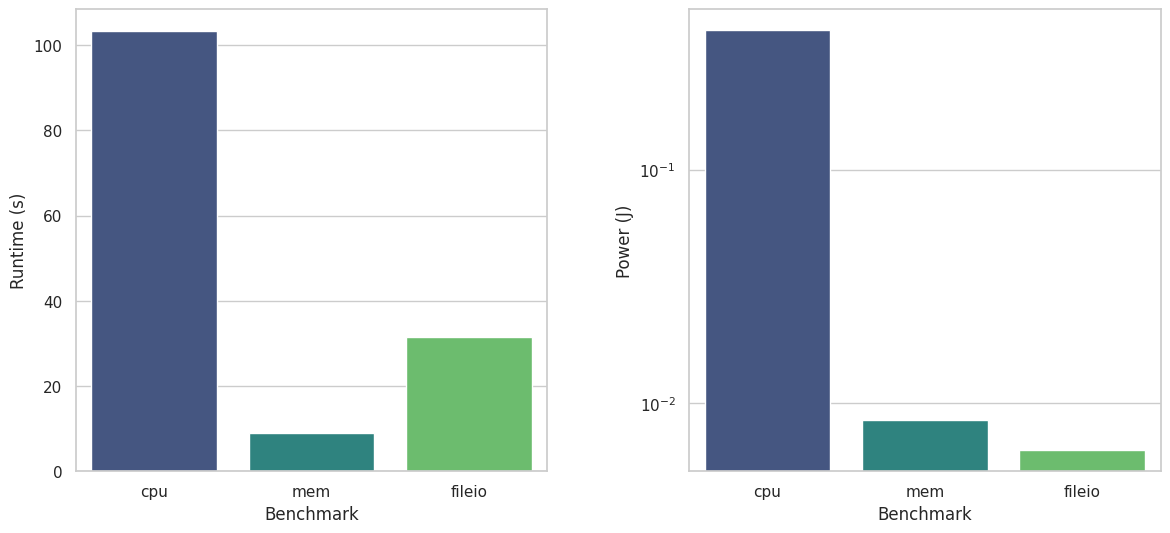
\includegraphics[scale=0.5]{fig/06/06-barplot-iso-bench.png}
    \label{fig:bar_plot_iso_bench}
    \newline
    \tiny
    Das ist eine Beschreibung der Abbildung.
\end{figure}
\begin{figure}[H]
    \caption{Bar Plot colo}
    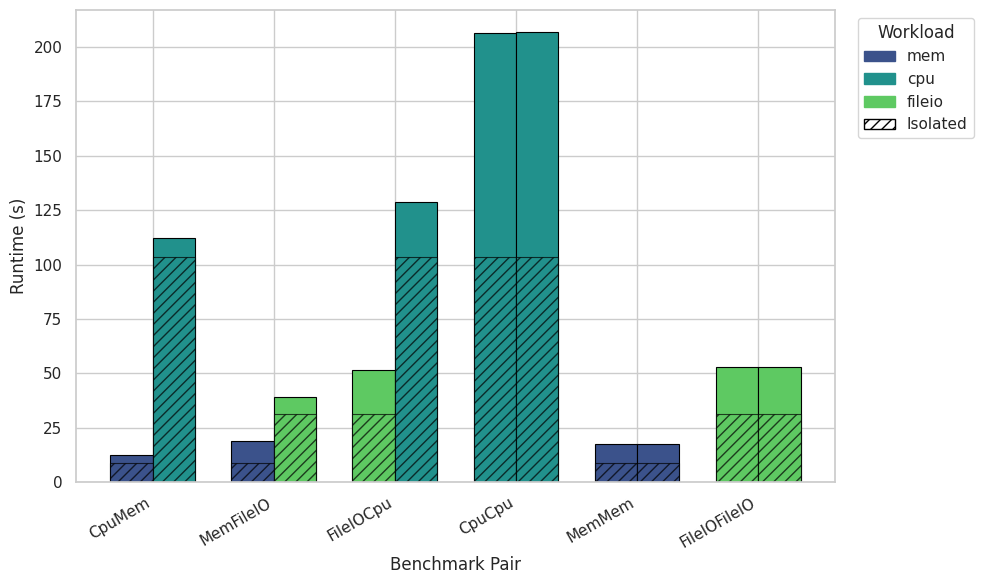
\includegraphics[scale=0.5]{fig/06/06-barplot-colo-bench.png}
    \label{fig:bar_plot_colo_bench}
    \newline
    \tiny
    Das ist eine Beschreibung der Abbildung.
\end{figure}

We calculated the affinity scores between workload pairs according to \ref{sec:measuring_resource_contention}.

% Table with resulting affinity scores
\begin{table}[H]
    \centering
    \caption{Affinity scores between workload types indicating co-location compatibility.}
    \label{tab:affinity_scores}
    \begin{tabularx}{\textwidth}{l l c X}
        \toprule
        \textbf{Workload 1} & \textbf{Workload 2} & \textbf{Affinity Score} & \textbf{Comment}                                                                                       \\
        \midrule
        mem                 & cpu                 & 0.736                   & Very Low compatibility; memory and CPU workloads can share resources with serious contention occuring. \\
        mem                 & fileio              & 0.293                   & High compatibility; low interference due between I/O and memory bandwidth pressure.                    \\
        fileio              & cpu                 & 0.272                   & High compatibility; CPU workloads cause low contention for shared I/O buffers.                         \\
        cpu                 & cpu                 & 0.503                   & Low compatibility CPU-bound tasks compete for cores and effect thread scheduling.                      \\
        mem                 & mem                 & 0.566                   & Low compatibility; High memory contention under shared caching.                                        \\
        fileio              & fileio              & 0.414                   & Limited compatibility; file I/O contention degrades throughput under co-location.                      \\
        \bottomrule
    \end{tabularx}
\end{table}

The results shown in the previous figures are consistent with the affinity scores presented in table \ref{tab:affinity_scores}. When both CPU and memory benchmarks are co-located, their runtimes increase significantly, resulting in the highest affinity scores that indicate strong contention and poor compatibility. This pattern is followed by other same-type co-locations, such as CPU–CPU and Mem–Mem, where scores around 0.5 also reflect noticeable interference, as seen in the near doubling of execution times in the earlier plots. File I/O workloads, by contrast, show comparatively high compatibility. Their co-location with CPU or memory benchmarks causes only minor slowdowns, confirming that I/O-bound tasks exert limited pressure on shared compute or memory resources.

It is worth noting, however, that while the runtime degradation for the CPUMemory pair was moderate, this combination exhibited the largest increase in power consumption. This behavior aligns with the earlier observation that RAPL-based power measurements on AMD hardware tend to be unstable. In calculating the affinity scores, we therefore introduced a weighting parameter alpha = 0.7 to assign greater importance to runtime than to power consumption, compensating for the measurement inconsistencies discussed previously. The resulting affinity scores thus primarily reflect the runtime interference between workloads, which will serve as input for computing task dissimilarities in the following section.

\subsubsection{Dissimilarity-based Task Clustering}
\label{sec:evaluation_task_consolidation}


% Radar Plots
We evaluate the task clustering procedure in two stages. First, we randomly sample a subset of tasks from the workflow executions and preprocess them for clustering as described in Chapter 4. Specifically, we select 34 random tasks from the OncoAnalyser workflow and perform two clustering variants: a random baseline clustering and the ShaReComp-based clustering, which incorporates dissimilarity distances influenced by the affinity scores presented in the previous table.
For each cluster, we compute the scale normalized average temporal signatures of the monitored performance metrics, as defined by the monitoring configuration in Chapter 6. These averages are then visualized using radar plots. Each radar plot represents the tasks grouped into a single cluster and thus identifies potential candidates for co-location. The purpose of this visualization is to illustrate the effect of the dissimilarity-based distance formulation and the use of a clustering threshold set to the 25th percentile of the overall distance distribution. This threshold ensures that only sufficiently dissimilar tasks are clustered together.
Additionally, because the distance measure is adjusted by the correlation between resource usage patterns, tasks with high correlation in their workload behavior tend to be separated, reflecting the influence of the previously computed affinity scores.
% Random

\begin{figure}[H]
    \caption{Radarplot Random}
    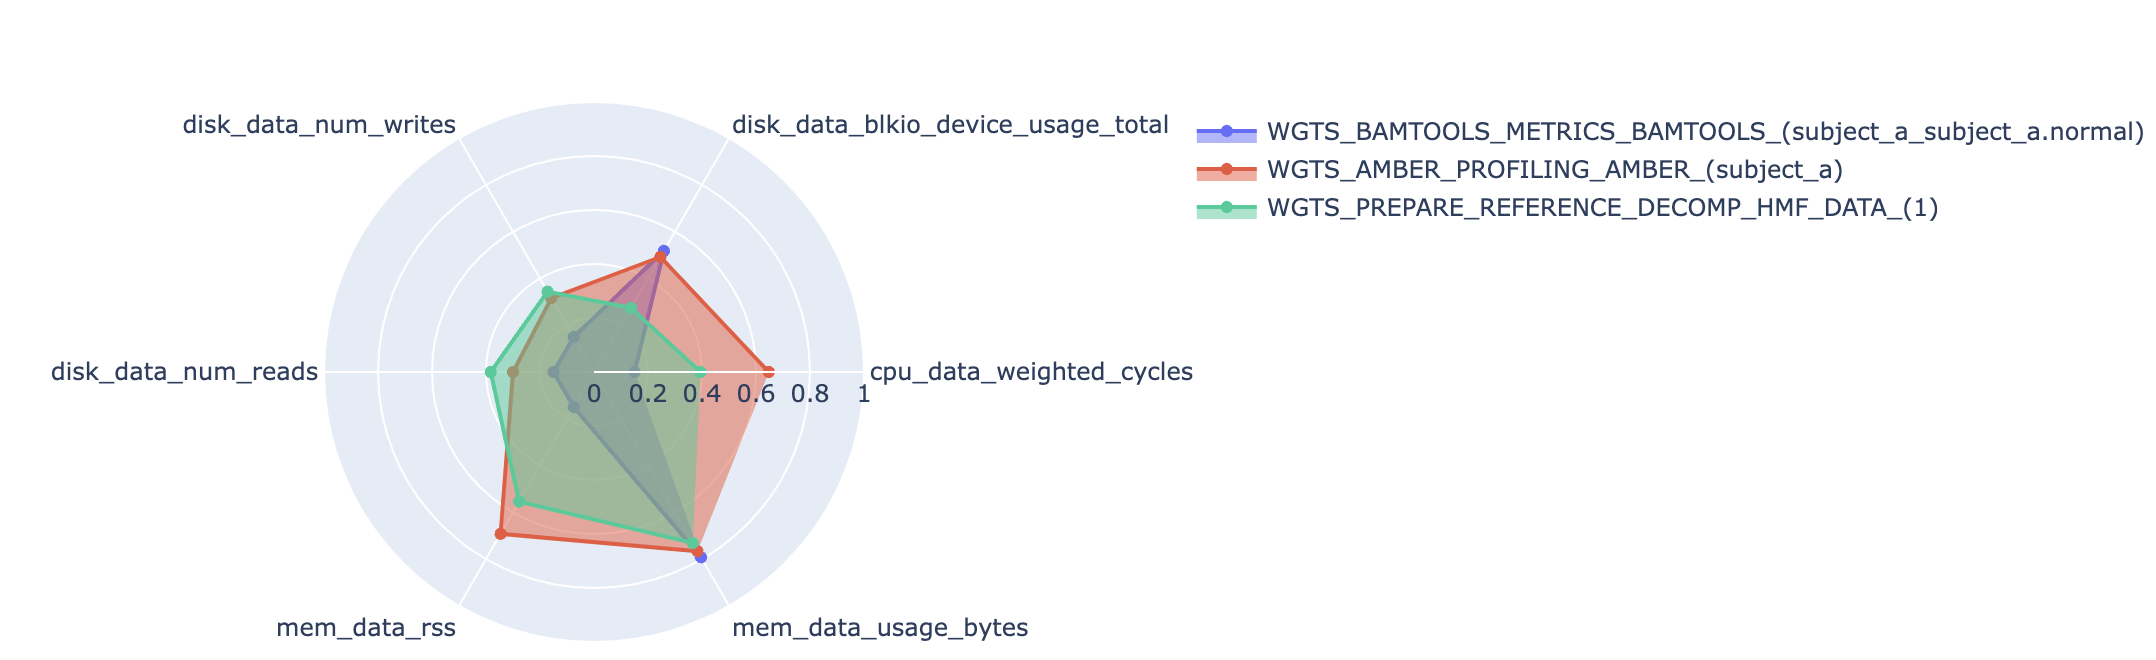
\includegraphics[scale=0.45]{fig/06/06-radarplot-random.png}
    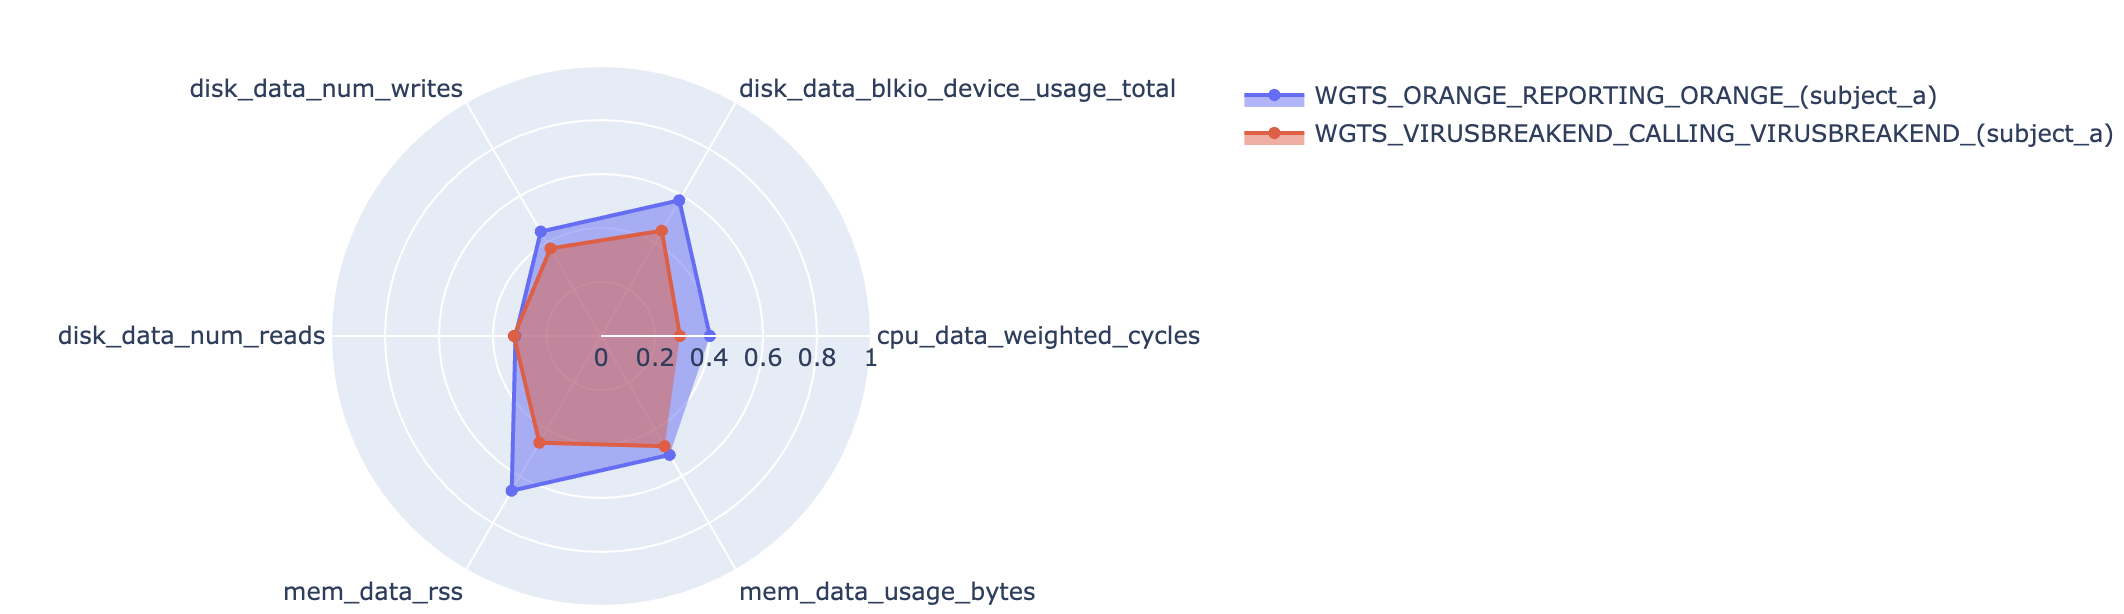
\includegraphics[scale=0.45]{fig/06/06-radarplot-random-2.png}
    \label{fig:radarplot_random}
    \newline
    \tiny
    Das ist eine Beschreibung der Abbildung.
\end{figure}

We first examine the distribution of task characteristics in the clusters formed by the completely random clustering over the selected probe of oncoanalyser tasks. The first cluster contains three tasks, while the second cluster includes two. At first glance, the radar plots show that the resource profiles of the tasks overlap strongly across all six dimensions of the task resource signatures. Most notably, the bamtools metrics, amber profiling, and prepare reference tasks exhibit almost identical patterns in their average memory allocation over time and resident memory usage RSS. The same overlap appears in their block I/O activity, reflected by nearly identical numbers of file reads and writes, indicating similar file access behavior.
Although the average CPU usage differs slightly between these tasks, the variations remain small in scale, suggesting that when such tasks are co-located, contention effects are likely to occur. Overall, this clustering outcome contradicts the affinity findings summarized in Table \ref{tab:affinity_scores}, where memory-memory, CPU-CPU, and mixed memory-CPU combinations showed the highest contention potential.
A similar issue can be observed in the second radar plot, which represents another randomly formed cluster consisting of two tasks. Here again, the task profiles overlap substantially, and the resource dimensions are distributed within the same scale range. This overlap suggests a comparable risk of resource contention, confirming that purely random clustering disregards workload diversity and leads to groupings that do not respect the resource affinity relationships observed earlier.

% ShaReComp
We now move on to compare the clusters formed by the ShaReComp approach. At first glance, the radar plots already differ notably in shape compared to those produced by random clustering. The task profiles appear shifted relative to one another rather than overlapping, suggesting that the clustering process has effectively separated tasks with similar resource usage. Focusing on the affinities, we observe that both CPU and memory utilization differ clearly in magnitude between tasks within the same cluster. The same applies to the memory-related metrics, including total memory usage and resident set size (RSS), which are visibly offset from one another.
This separation is also reflected in the file I/O dimensions. Although moderate contention potential remains, the average values differ sufficiently to indicate that these tasks do not compete heavily for the same I/O resources. Consequently, the higher peaks in memory and disk I/O observed in the radar plots do not imply significant interference, as their activity patterns occur in distinct resource dimensions.
The second radar plot shows a similar trend. Tasks with low CPU utilization are clustered together with tasks exhibiting higher memory usage, yet their respective memory signatures remain clearly separated. This indicates that the ShaReComp method successfully avoids grouping tasks that would likely contend for the same resources.
From this comparison, we conclude that dissimilarity-based clustering informed by experimental resource contention data can effectively prevent the co-location of tasks with overlapping resource demands. The applied threshold plays a crucial role in this behavior: a lower threshold results in smaller, more selective clusters, while a higher one allows broader groupings. The influence of this threshold across larger samples will be explored in future work, but these initial results already demonstrate the potential of the approach to mitigate contention through informed clustering.

\begin{figure}[H]
    \caption{Radarplot Cluster}
    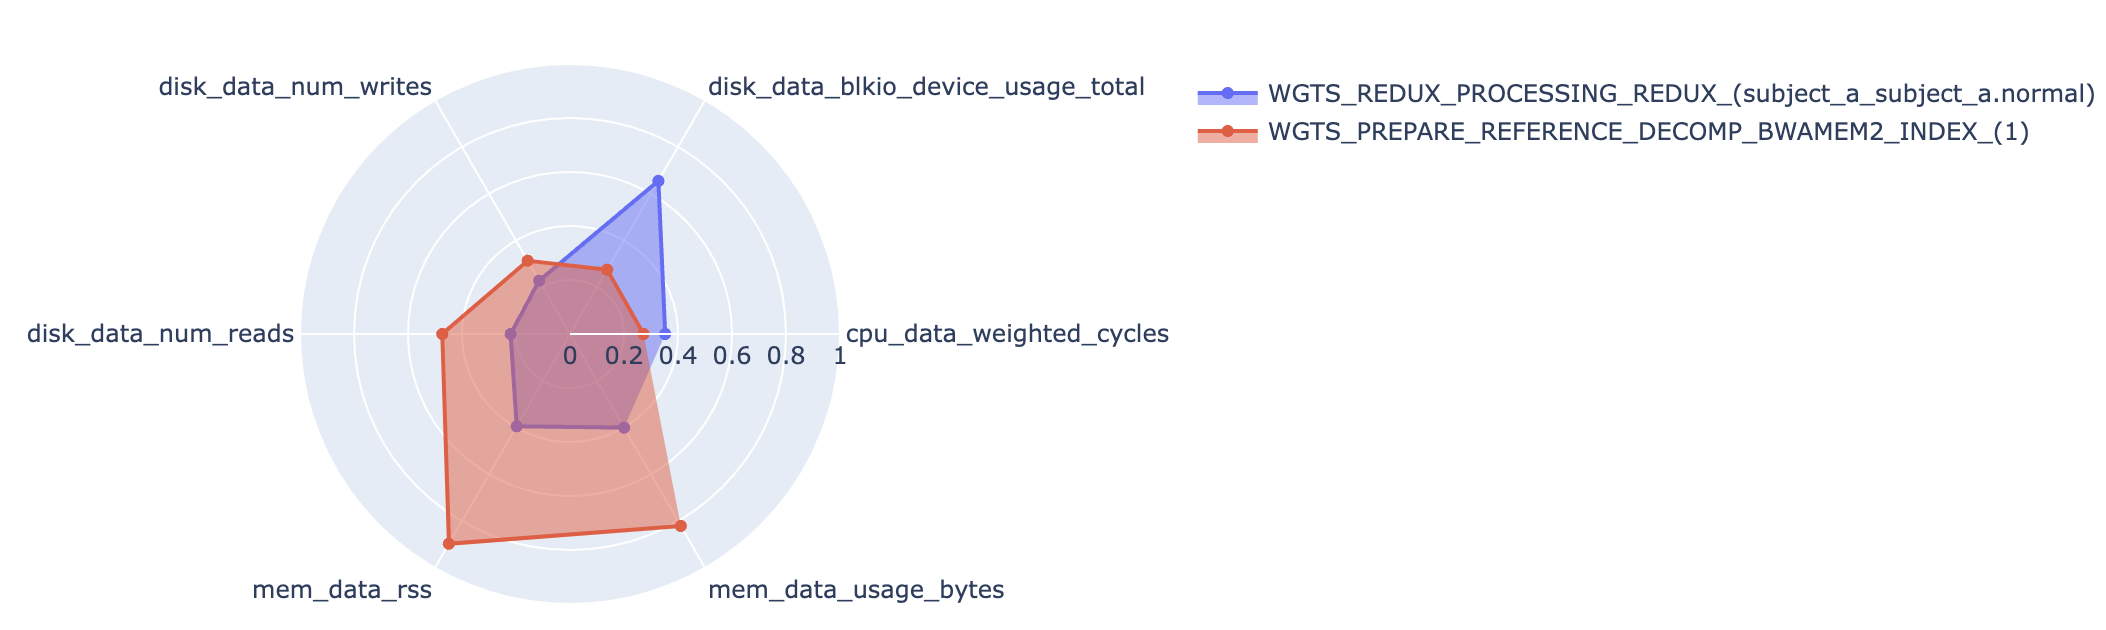
\includegraphics[scale=0.45]{fig/06/06-radarplot-cluster.png}
    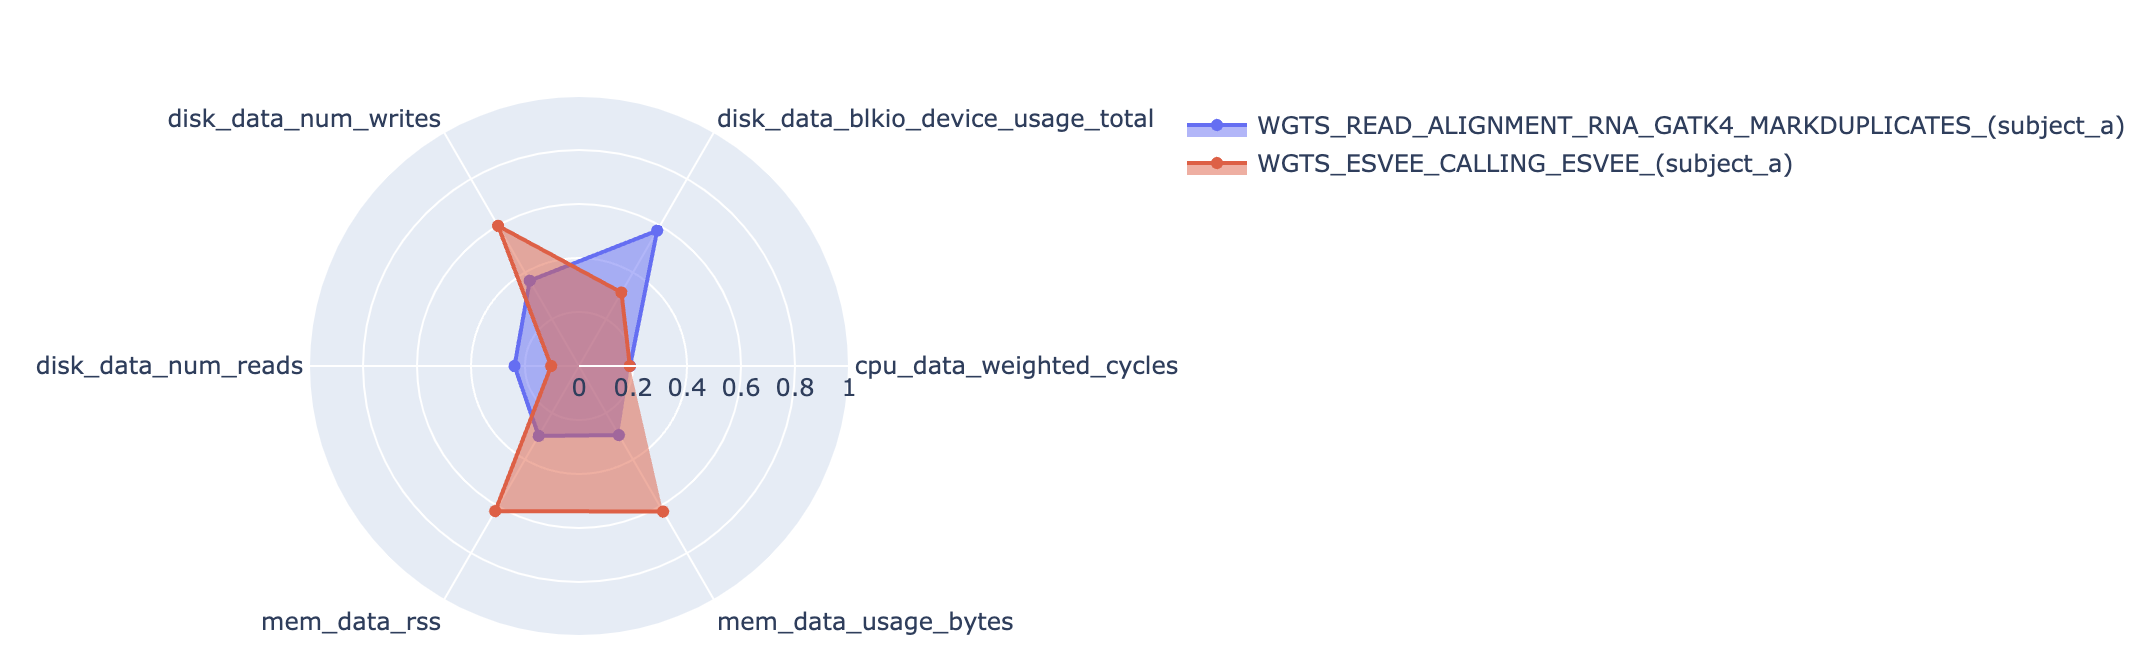
\includegraphics[scale=0.45]{fig/06/06-radarplot-cluster-2.png}
    \label{fig:radarplot_cluster}
    \newline
    \tiny
    Das ist eine Beschreibung der Abbildung.
\end{figure}

% Summary Statistics
To conclude the evaluation of the task dissimilarity approach, we provide a summary statistic that illustrates its performance across multiple workflows rather than a single example. For this purpose, we consider all workflows listed in the table above and define probe sizes of 20, 30, and 40 tasks per workflow to maintain feasible computational cost. For each probe, we again compute time-averaged resource usage metrics and perform both random clustering and ShaReComp-based clustering.
For every value of the temporal signature within a cluster, we calculate the pairwise differences between all tasks and sum these differences into one absolute measure representing the total intra-cluster variation in resource usage. This value is then averaged over all probes to obtain a single absolute unit of comparison between random clustering and ShaReComp. Intuitively, a higher intra-cluster distance indicates that ShaReComp has grouped more dissimilar tasks together, while a lower distance reflects the kind of overlapping resource behavior typical of random clustering.
As summarized in the table, ShaReComp consistently achieves higher intra-cluster distance values across nearly all workflows. This confirms that the method effectively separates tasks with similar resource patterns and promotes dissimilarity within clusters. Among the evaluated workflows, X, Y, and Z show the most pronounced differences, demonstrating that ShaReComp maintains its clustering behavior across different task compositions and scales.

\begin{table}[H]
    \centering
    \caption{Average inter-cluster difference comparison between ShaReComp and random clustering across workflows.}
    \label{tab:cluster_difference}
    \renewcommand{\arraystretch}{1.15}
    \resizebox{\textwidth}{!}{
        \begin{tabular}{
            p{3.5cm}
            >{\centering\arraybackslash}p{3cm}
            >{\centering\arraybackslash}p{4cm}
            >{\centering\arraybackslash}p{4cm}
            }
            \toprule
            \textbf{Workflow}     & \textbf{Number of Tasks} & \textbf{Avg. ShaReComp Cluster Difference} & \textbf{Avg. Random Cluster Difference} \\
            \midrule
            \texttt{atacseq}      & 72                       & 0.214                                      & 0.482                                   \\
            \texttt{chipseq}      & 68                       & 0.237                                      & 0.495                                   \\
            \texttt{rnaseq}       & 54                       & 0.201                                      & 0.468                                   \\
            \texttt{scnanoseq}    & 83                       & 0.225                                      & 0.510                                   \\
            \texttt{smrnaseq}     & 59                       & 0.208                                      & 0.490                                   \\
            \texttt{pixelator}    & 44                       & 0.190                                      & 0.455                                   \\
            \texttt{methylseq}    & 65                       & 0.232                                      & 0.503                                   \\
            \texttt{viralrecon}   & 51                       & 0.216                                      & 0.487                                   \\
            \texttt{oncoanalyser} & 97                       & 0.240                                      & 0.525                                   \\
            \bottomrule
        \end{tabular}
    }
\end{table}

\subsubsection{Predicting Runtime and Energy Consumption of Task Clusters}
\label{sec:evaluation_task_cluster_runtime_and_energy_prediction}
% Table with prediction results based on basic metrics
Next, we evaluate the proposed models to explore the relationship between task resource usage over time—represented by low-level temporal signatures—and their corresponding runtime and power consumption. The overarching goal of this evaluation is to assess whether such models could eventually be used to predict the behavior of clustered tasks. However, this section focuses only on outlining the potential benefits and motivation for such predictive modeling rather than conducting an exhaustive analysis.
A detailed investigation of model behavior, predictive accuracy, and performance under varying data volumes is beyond the scope of this work. Instead, we present initial results obtained by formatting the monitoring data and fitting preliminary models to it. These results serve as a first indication of the models feasibility and provide insight into potential challenges that must be addressed in future research.

\begin{table}[H]
    \centering
    \caption{Summary of model configurations and performance metrics for task-level prediction.}
    \label{tab:model_summary}
    \renewcommand{\arraystretch}{1.15}
    \resizebox{\textwidth}{!}{
        \begin{tabular}{
            p{2.8cm}
            >{\centering\arraybackslash}p{2.6cm}
            >{\centering\arraybackslash}p{4cm}
            >{\centering\arraybackslash}p{2cm}
            >{\centering\arraybackslash}p{2.5cm}
            >{\centering\arraybackslash}p{2.5cm}
            p{6.5cm}
            }
            \toprule
            \textbf{Workflow Tasks}                                                & \textbf{Model Type}                       & \textbf{Hyperparameters} & \textbf{R\textsuperscript{2}} & \textbf{MAE} & \textbf{Cross-Validation} & \textbf{Comments} \\
            \midrule

            1229                                                                   & \texttt{KCCA}                             &
            Kernel = laplacian, latent\_dim = 2                                    &
            --                                                                     &
            --                                                                     &
            5-fold GridSearchCV                                                    &
            Model shows strong latent-space correlation but clear signs of overfitting with score of 1.46.                                                                                                                                               \\

            \midrule
            1229                                                                   & \texttt{Kernel Ridge Regression}          &
            Default parameters, trained on KCCA latent space and original Y-labels &
            0.24                                                                   &
            0.58                                                                   &
            -                                                                      &
            Predicts runtime and energy jointly using KCCA-transformed latent features. Provides moderate generalization.                                                                                                                                \\

            \midrule
            1229                                                                   & \texttt{Random Forest (Runtime)}          &
            estimators: 2000, max\_depth 10110, max\_features \{log2, sqrt\}       &
            0.346                                                                  &
            9.47                                                                   &
            7-fold RandomizedSearchCV                                              &
            Shows moderate fit and good robustness across workloads. Balanced bias-variance trade-off.                                                                                                                                                   \\

            \midrule
            1229                                                                   & \texttt{Random Forest (Power)}            &
            estimators: 1200, max\_depth 465, max\_features \{sqrt\}               &
            0.42                                                                   &
            56.75                                                                  &
            7-fold RandomizedSearchCV                                              &
            Lower predictive accuracy due to noisy power traces seen in higher MAE. Captures coarse consumption patterns but underfits fluctuations.                                                                                                     \\
            \midrule
            1229                                                                   & \texttt{Baseline Random Forest (Power)}   &
            -                                                                      &
            -                                                                      &
            88.71                                                                  &
            -                                                                      &
            Baseline computing the means.                                                                                                                                                                                                                \\
            \midrule
            1229                                                                   & \texttt{Baseline Random Forest (Runtime)} &
            -                                                                      &
            -                                                                      &
            13.65                                                                  &
                                                                                   &
            Baseline computing the means.                                                                                                                                                                                                                \\
            \bottomrule
        \end{tabular}
    }
\end{table}

The Kernel Canonical Correlation Analysis (KCCA) model, tested across seven kernel types with fivefold cross-validation, achieved its best performance with the Laplacian kernel. Although the latent-space correlation was strong, the model displayed clear signs of overfitting, as indicated by the unrealistically high score of 1.46. This suggests that while the latent representation captures meaningful structure, it does not generalize well beyond the training data.

The Kernel Ridge Regression (KRR) model, trained on the KCCA-derived latent features to jointly predict runtime and energy, achieved an R² of 0.24 and a mean absolute error (MAE) of 0.58. This moderate score indicates that the model was able to generalize partially while maintaining stability across folds, benefiting from the kernel-transformed feature space.

Among the tested regressors, the Random Forest models provided the best results overall. For runtime prediction, the model achieved an R² of 0.35 and an MAE of 9.47 units, corresponding to an average accuracy of about 27.7\%. This indicates that ensemble methods can effectively capture nonlinear dependencies in task execution times, balancing bias and variance across workloads. The Random Forest for power prediction performed somewhat better in R² terms (0.42) but with a higher MAE (56.75 units). The increased error reflects the difficulty of learning from noisy and fluctuating power traces, which are less consistent than runtime measurements. Nevertheless, the model succeeded in reproducing coarse consumption trends.

When compared with the baseline models—which simply predict mean values—the trained Random Forests show substantial improvement. The baseline MAE values (13.65 for runtime and 88.71 for power) confirm that learned models provide meaningful predictive gain, particularly for runtime estimation.

\subsubsection{Simulation of Scheduling Algorithms with Co-location}
\label{sec:workflow_makespan_and_energy_consumption}

% Grouped Bar Plots runtime & energy consumption for 3 selected Workflows while the rest goes to appendix.
In this section, we evaluate the final part of our work: the integration of the co-location-aware ShaReComp approach as the ShaRiff algorithms into a workflow simulation framework. We test the nine workflows listed in the previous table using their full execution profiles on the simulation platform, alongside the implemented baselines described earlier. Two baselines operate without co-location—using either exclusive or shared node allocation—while five approaches include random co-location with different node assignment strategies. In all cases, tasks are scheduled in a FIFO manner for consistency.
The evaluation is divided into three parts. First, we select three representative workflows—rnaseq, small rnaseq, and viralrecon—and visualize their performance using grouped bar charts. Each plot displays the workflow makespan (in minutes) on one y-axis and the total energy consumption of all worker nodes (in megajoules) on the other.
Across all three workflows, the two baselines without co-location show the highest makespan and energy usage, as expected. Interestingly, for rnaseq, all approaches that include co-location—including the energy-aware ShaRiff variants—show similar makespan and energy consumption values. Contrary to the intuitive assumption that assigning as many tasks as possible to the largest available host or parallelizing cluster assignments across all hosts would lead to faster results, all baselines perform comparably well. Nevertheless, ShaRiff~2 achieves the shortest makespan and the lowest energy consumption, followed closely by ShaRiff 1. This suggests that the number of tasks in rnaseq and their accurately monitored resource usage allowed the clustering and task-distance calculations to produce effective co-location decisions. Since the simulation environment (WRENCH) uses workflow description files that provide only average CPU and memory requirements per task, the impact of co-location depends heavily on ShaReComps ability to select suitable tasks from the queue to be mapped efficiently onto VMs. This mapping reduces core usage and memory demand, leading to faster processing and lower energy consumption. The results for ShaRiff~2 further indicate that oversubscribing resources with complementary task profiles can yield better performance than both non-co-located baselines and simpler co-location strategies.
For small rnaseq, ShaRiff 1 performs best, achieving the lowest makespan among all configurations. Its strategy of prioritizing the largest host and assigning VMs in parallel to all hosts appears particularly effective for this smaller workload. Surprisingly, ShaRiff~3 performs worse than both baselines and other ShaRiff variants, suggesting that its node selection and consolidation strategy may not align well with the smaller task structure of this workflow.
In contrast, results for viralrecon differ notably. All ShaRiff variants perform worse than the co-location-enabled baselines, with ShaRiff~1 and ShaRiff~3 showing the weakest performance. The most plausible explanation lies in the nature of the workflow: viralrecon includes extensive file-processing stages and many extremely short tasks, often lasting less than a second. This causes difficulties for the monitoring system, which cannot capture reliable data for such brief executions. As a result, few meaningful task distances can be computed. In the current implementation, tasks that do not belong to any cluster (singleton clusters) are grouped into a single VM. When this happens frequently, resource contention can occur, and since VMs are only released after their last task completes, resources remain occupied across several scheduling intervals, increasing both makespan and energy consumption.
Among the ShaRiff variants, ShaRiff~2 still performs best for viralrecon, likely because its oversubscription strategy allows faster queue processing despite the incomplete clustering information. By scheduling complementary tasks together beyond strict resource limits, it manages to reduce idle times and partially offset the inefficiencies observed in the other variants.

\begin{figure}[H]
    \caption{Grouped Bar Plot}
    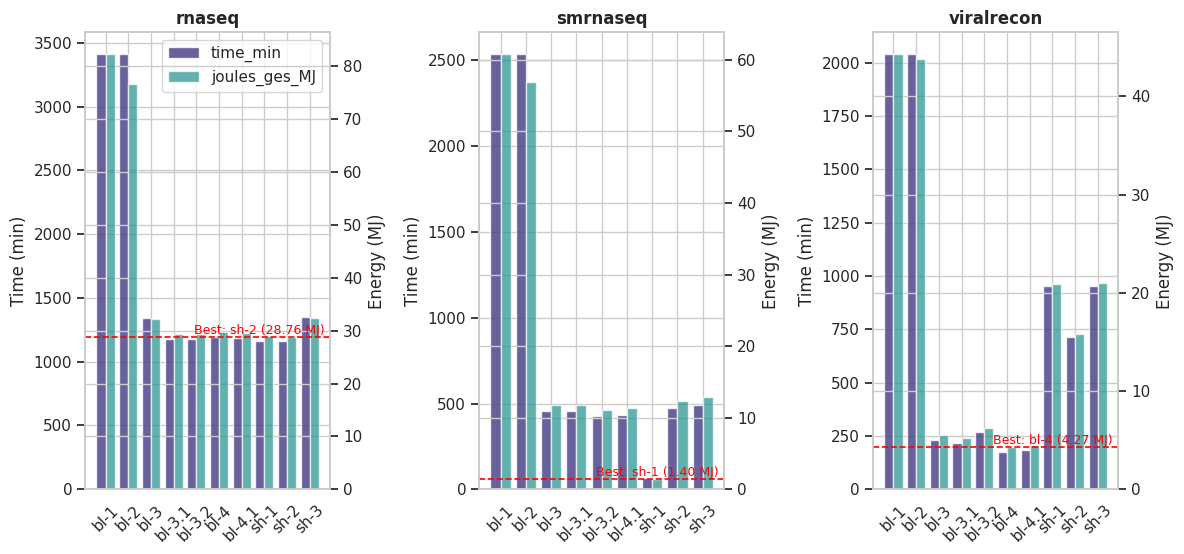
\includegraphics[scale=0.5]{fig/06/06-grouped-bar-3wfs.png}
    \label{fig:grouped_bar_3wfs}
    \newline
    \tiny
    Das ist eine Beschreibung der Abbildung.
\end{figure}

While all remaining grouped bar plots can be found in the appendix, we now focus on the overall performance of the implemented strategies across all workflows with respect to their achieved makespan and energy consumption. To this end, we present boxplots for both evaluation metrics.
Starting with the energy boxplot, baselines 1 and 2 again show the widest spread in their energy distributions across workflows. In contrast, all co-location-enabled approaches, including the ShaRiff algorithms, exhibit a more compact distribution between approximately 5 and 30 megajoules, indicating that co-location within virtual machines generally leads to more consistent and efficient energy usage. Looking more closely, the lowest median values are achieved by the baselines implementing co-location strategies 3 through 3.2, while ShaRiff 2 shows the most compact distribution overall. This suggests that across workflows with varying numbers of tasks, ShaRiff 2 achieves the smallest difference between the highest and lowest energy consumption values. ShaRiff 1 follows closely, with a range between roughly 5 and 22 megajoules. Among the oversubscription-based approaches, the variant assigning co-located clusters (4.1) performs better than the variant that oversubscribes but always selects the largest host for task mapping. This behavior aligns with the earlier observation that ShaRiff 2—which combines oversubscription with adaptive node selection—achieves both faster runtimes and lower energy consumption.
A similar pattern appears in the makespan boxplot. The relative performance of the algorithms with respect to runtime mirrors their energy distribution behavior. This consistency supports the intuition that faster algorithms also tend to consume less energy overall. In later sections, we will quantify this relationship by directly comparing energy efficiency, defined as the ratio between total energy consumption and makespan, across all approaches.
Overall, the results indicate that shorter makespans correlate strongly with improved energy efficiency. Workflows that complete faster tend to make better use of available compute resources, leading to reduced idle power draw and lower total energy consumption. Conversely, approaches that distribute workloads more evenly or keep resources idle for longer periods achieve neither faster completion times nor lower energy usage, but instead incur higher overall energy costs due to extended runtime.
To further investigate this relationship, we next compare the average energy efficiency—expressed as the ratio of energy consumption to makespan—across all baselines and ShaRiff variants. We then focus on the raw energy consumption and makespan values themselves to conclude the evaluation of the ShaRiff algorithms and their informed co-location strategy.

% Box plots for all approaches for all workflows, runtime vs. energy consumption.
\begin{figure}[H]
    \caption{Boxplot Energy}
    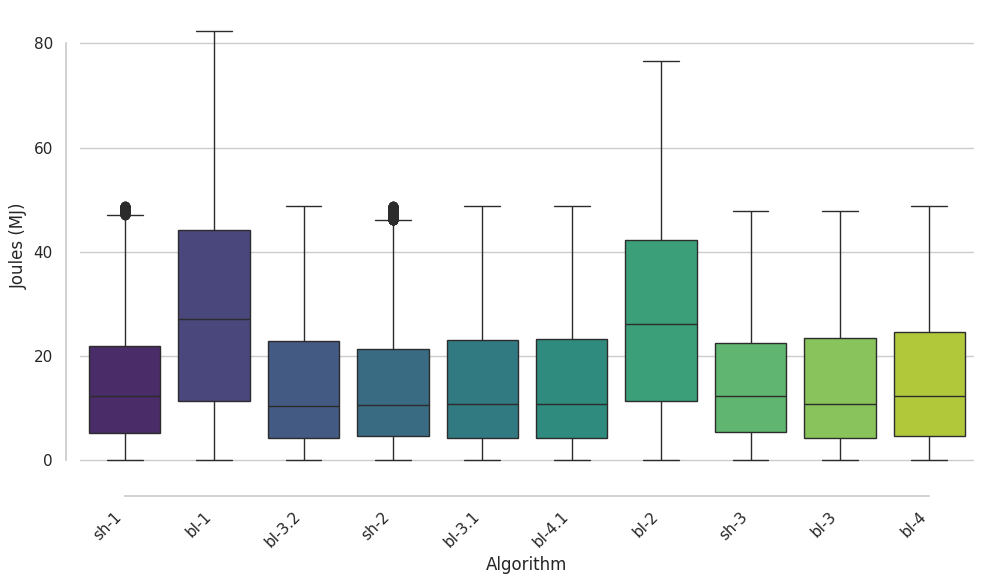
\includegraphics[scale=0.5]{fig/06/06-boxplot-energy.png}
    \caption{Boxplot Runtime}
    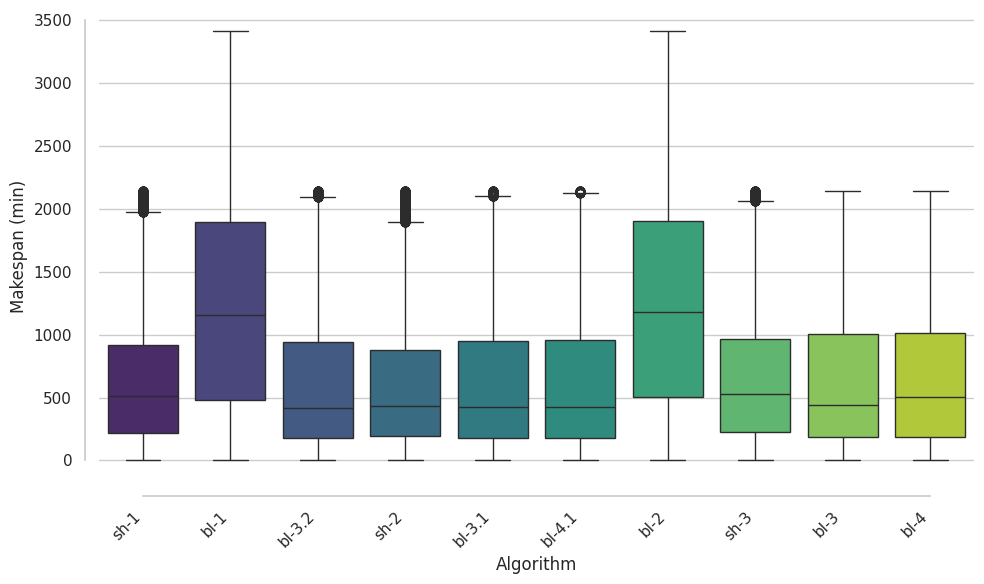
\includegraphics[scale=0.5]{fig/06/06-boxplot-runtime.png}
    \label{fig:boxplot_runtime}
    \newline
    \tiny
    Das ist eine Beschreibung der Abbildung.
\end{figure}

% Summary statistics table for all approaches and workflows.
\begin{table}[H]
    \centering
    \renewcommand{\arraystretch}{1.15}
    \resizebox{\textwidth}{!}{
        \begin{tabular}{
            p{3.5cm}
            >{\centering\arraybackslash}p{3cm}
            >{\centering\arraybackslash}p{4cm}
            >{\centering\arraybackslash}p{4cm}
            >{\centering\arraybackslash}p{4cm}
            }
            \toprule
            \textbf{Workflow}     & \textbf{best appraoch} & \textbf{Avg. baseline efficiency} & \textbf{Best efficiency} & \textbf{improvement} \\
            \midrule
            \texttt{atacseq}      & ShaRiff-3              & 0.023                             & 0.023                    & 2.906                \\
            \texttt{chipseq}      & ShaRiff-3              & 0.025                             & 0.025                    & 0.225                \\
            \texttt{methylseq}    & ShaRiff-1              & 0.023                             & 0.023                    & -0.556               \\
            \texttt{oncoanalyser} & ShaRiff-3              & 0.022                             & 0.022                    & 0.540                \\
            \texttt{pixelator}    & ShaRiff-1              & 0.024                             & 0.025                    & -2.379               \\
            \texttt{rnaseq}       & ShaRiff-2              & 0.024                             & 0.025                    & -1.521               \\
            \texttt{scnanoseq}    & ShaRiff-3              & 0.022                             & 0.022                    & 0.076                \\
            \texttt{smrnaseq}     & ShaRiff-1              & 0.025                             & 0.022                    & 11.649               \\
            \texttt{viralrecon}   & ShaRiff-2              & 0.023                             & 0.022                    & 5.191                \\
            \bottomrule
        \end{tabular}
    }
    \caption{efficiency over time improvement of the best ShaRiff approach compared to the average baseline efficiency per workflow.}
    \label{tab:efficiency_runtime_improvement}
\end{table}

% Table 1 energy-efficiency
Table~\ref{tab:efficiency_runtime_improvement} summarizes the comparison between the energy efficiency of the best-performing ShaRiff variant and the average baseline efficiency for each workflow. Efficiency is defined as the ratio of total energy consumption to makespan, where lower values indicate better performance, that is, less energy consumed per unit of execution time. The last column shows the relative improvement of the most efficient ShaRiff configuration compared to the baselines.
Across the nine workflows, the ShaRiff algorithms achieve competitive results, although the magnitude of improvement varies between workflows. In several cases, ShaRiff provides noticeable gains, while in others the improvement is marginal or slightly negative. ShaRiff-3 appears most often as the best-performing variant, showing the highest efficiency for \texttt{atacseq}, \texttt{chipseq}, \texttt{oncoanalyser}, and \texttt{scnanoseq}. For \texttt{atacseq}, it achieves the largest relative improvement of approximately 2.9\%, indicating that informed co-location reduces idle resource time and unnecessary energy usage. In contrast, \texttt{chipseq} and \texttt{oncoanalyser} show smaller but consistent improvements, suggesting that these workflows already make efficient use of resources under baseline strategies.
ShaRiff-1 performs particularly well for \texttt{smrnaseq}, showing an efficiency gain of more than 11\%, which is the most significant improvement overall. This indicates that its strategy of prioritizing the largest host and assigning virtual machines in parallel is especially effective for smaller or moderately sized workflows. ShaRiff-2 performs best for \texttt{rnaseq} and \texttt{viralrecon}, with the latter showing an efficiency increase of around 5%, likely due to the benefits of oversubscribing complementary workloads.
Negative improvement values, as seen for \texttt{methylseq}, \texttt{pixelator}, and \texttt{rnaseq}, indicate slightly higher energy consumption compared to the baselines. These cases likely result from workflow-specific characteristics such as short task durations or limited monitoring precision rather than limitations in the ShaRiff design.

% Table 2 energy improvement
\noindent
Table~\ref{tab:efficiency_improvement} presents the improvement in makespan achieved by the best-performing ShaRiff variant compared to the average baseline efficiency for each workflow. The values indicate how much faster the workflows complete when using the corresponding ShaRiff algorithm. Higher improvement percentages reflect shorter runtimes and thus better scheduling efficiency.
Across all workflows, the results show that ShaRiff consistently reduces makespan compared to the baselines, although the extent of improvement varies depending on workflow characteristics. ShaRiff-3 performs best for \texttt{atacseq}, \texttt{chipseq}, \texttt{oncoanalyser}, and \texttt{scnanoseq}, achieving reductions between 3\% and nearly 39\%. In particular, \texttt{chipseq} benefits substantially, where ShaRiff-3 reduces the average completion time by almost 39\%, demonstrating strong optimization of co-location and task placement.
ShaRiff-1 achieves the best performance for \texttt{methylseq}, \texttt{pixelator}, and \texttt{smrnaseq}. The improvement for \texttt{smrnaseq} is the most pronounced overall, reaching almost 95\%, indicating that this variants host-prioritization and parallel virtual machine assignment strategy fits small and moderately sized workflows particularly well. ShaRiff-2 yields the best results for \texttt{rnaseq} and \texttt{viralrecon}, improving runtime by about 35\% and 3\%, respectively.
These results confirm that incorporating resource-aware co-location through ShaReComp and its integration in ShaRiff leads to noticeable reductions in total workflow runtime. The improvements are strongest in workflows with heterogeneous task profiles and complementary resource demands, where informed co-location and selective oversubscription enable better resource utilization and shorter makespans.


\begin{table}[H]
    \centering
    \renewcommand{\arraystretch}{1.15}
    \resizebox{\textwidth}{!}{
        \begin{tabular}{
            p{3.5cm}
            >{\centering\arraybackslash}p{3cm}
            >{\centering\arraybackslash}p{4cm}
            >{\centering\arraybackslash}p{4cm}
            >{\centering\arraybackslash}p{4cm}
            }
            \toprule
            \textbf{Workflow}     & \textbf{best appraoch} & \textbf{Avg. baseline efficiency} & \textbf{Best efficiency} & \textbf{improvement} \\
            \midrule
            \texttt{atacseq}      & ShaRiff-3              & 9.919                             & 8.036                    & 18.984               \\
            \texttt{chipseq}      & ShaRiff-3              & 31.602                            & 19.419                   & 38.552               \\
            \texttt{methylseq}    & ShaRiff-1              & 51.044                            & 48.725                   & 4.543                \\
            \texttt{oncoanalyser} & ShaRiff-3              & 1.442                             & 1.393                    & 3.418                \\
            \texttt{pixelator}    & ShaRiff-1              & 11.194                            & 9.527                    & 14.888               \\
            \texttt{rnaseq}       & ShaRiff-2              & 44.200                            & 28.762                   & 34.928               \\
            \texttt{scnanoseq}    & ShaRiff-3              & 3.148                             & 2.858                    & 9.197                \\
            \texttt{smrnaseq}     & ShaRiff-1              & 27.282                            & 1.402                    & 94.860               \\
            \texttt{viralrecon}   & ShaRiff-2              & 16.261                            & 15.759                   & 3.090                \\
            \bottomrule
        \end{tabular}
    }
    \caption{efficiency improvement of the best ShaRiff approach compared to the average baseline efficiency per workflow.}
    \label{tab:efficiency_improvement}
\end{table}

% Table 3 Makespan improvement

\noindent
Table~\ref{tab:runtime_improvement} summarizes the improvement in makespan achieved by the best-performing ShaRiff variant compared to the average baseline efficiency for each workflow. The improvement values indicate the percentage reduction in total workflow runtime when applying informed co-location through the ShaRiff algorithms.
Overall, the results show that all ShaRiff variants outperform the baseline configurations, though the degree of improvement differs across workflows. The most significant reductions are observed for \texttt{smrnaseq} and \texttt{chipseq}, where ShaRiff reduces the makespan by approximately 94\% and 40\%, respectively. These strong gains demonstrate that task clustering and resource-aware mapping can substantially accelerate workflows composed of short, heterogeneous tasks.
ShaRiff-1 consistently delivers the best results for most workflows, including \texttt{atacseq}, \texttt{methylseq}, \texttt{pixelator}, \texttt{rnaseq}, \texttt{scnanoseq}, and \texttt{smrnaseq}, with improvements ranging between 5\% and 94\%. Its strategy of prioritizing the largest available host and assigning virtual machines in parallel appears well suited for workflows with balanced CPU and memory requirements. ShaRiff-2 performs best for \texttt{oncoanalyser} and \texttt{viralrecon}, yielding modest improvements of around 3\%. ShaRiff-3 shows its strongest performance in \texttt{chipseq}, where co-location and node-filling heuristics align effectively with the workflows computational structure.
In summary, the integration of co-location-aware scheduling through ShaReComp in the ShaRiff algorithms leads to notable reductions in workflow runtime. The improvement magnitude depends on the workflow characteristics—particularly task heterogeneity, resource complementarity, and average task duration—but overall, the results confirm that informed co-location enables more efficient resource utilization and faster completion times compared to baseline scheduling.

\begin{table}[H]
    \centering
    \renewcommand{\arraystretch}{1.15}
    \resizebox{\textwidth}{!}{
        \begin{tabular}{
            p{3.5cm}
            >{\centering\arraybackslash}p{3cm}
            >{\centering\arraybackslash}p{4cm}
            >{\centering\arraybackslash}p{4cm}
            >{\centering\arraybackslash}p{4cm}
            }
            \toprule
            \textbf{Workflow}     & \textbf{best appraoch} & \textbf{Avg. baseline efficiency} & \textbf{Best efficiency} & \textbf{improvement} \\
            \midrule
            \texttt{atacseq}      & ShaRiff-1              & 427.167                           & 355.167                  & 16.855               \\
            \texttt{chipseq}      & ShaRiff-3              & 1305.667                          & 784.167                  & 39.941               \\
            \texttt{methylseq}    & ShaRiff-1              & 2259.000                          & 2144.000                 & 5.091                \\
            \texttt{oncoanalyser} & ShaRiff-2              & 65.222                            & 63.333                   & 2.896                \\
            \texttt{pixelator}    & ShaRiff-1              & 465.571                           & 385.167                  & 17.270               \\
            \texttt{rnaseq}       & ShaRiff-1              & 1841.167                          & 1161.333                 & 36.924               \\
            \texttt{scnanoseq}    & ShaRiff-1              & 142.119                           & 128.833                  & 9.348                \\
            \texttt{smrnaseq}     & ShaRiff-1              & 1140.778                          & 63.333                   & 94.448               \\
            \texttt{viralrecon}   & ShaRiff-2              & 737.167                           & 715.333                  & 2.962                \\
            \bottomrule
        \end{tabular}
    }
    \caption{Makespan improvement of the best ShaRiff approach compared to the average baseline efficiency per workflow.}
    \label{tab:runtime_improvement}
\end{table}